\documentclass[11pt]{article}
\usepackage{geometry}
 \geometry{
 a4paper,
 total={170mm,257mm},
 left=20mm,
 top=5mm,
 bottom=20mm
 }
\usepackage{graphicx} % Required for inserting images
\usepackage{caption}
\usepackage{tabularx}
\usepackage{booktabs} % for creating horizontal lines in tables
\usepackage{rotating} % for sideways table
%\usepackage{multirow}
 
\title{Figures and Tables}
\author{Narender Reddy}
\date{February 2025}

\begin{document}

\maketitle

\textbf{DISCLAIMER: All the data and figures shown in this work are from my PhD thesis and should be used as a template to create your own tables or figures.}

\section{Two figures in a single row using minipage}

This section shows the usage of minipages for depicting two figures side by side. This will help in presenting the results professionally. 


\subsection{Example 1}

This example shows only the figure number in the caption. The example also shows the use of the degree symbol, bold text, and delta symbol in the text. See how the height of the figures is used to align the figure and caption.

\vspace{0.5ex}

\begin{minipage}[c]{0.45\textwidth}
      \centering
      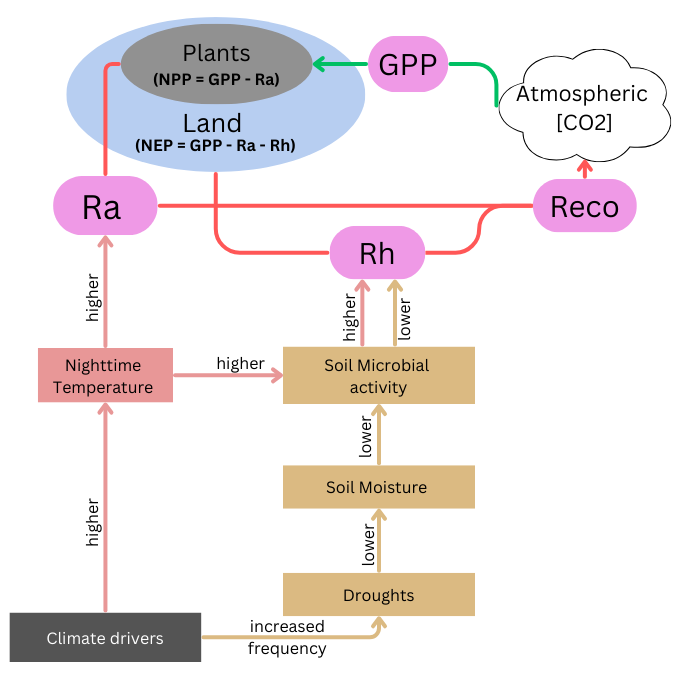
\includegraphics[height=2.4in]{Figures/Schematic_impact_on_carbon_fluxes_due_to_climate_24Oct.png}
      \captionof{figure}{Schematic showing uptake of CO$_{2}$ by plants (GPP) and ecosystem respiration (R$_{eco}$) combination of respiration from plants (R$_{a}$) and the land (R$_{h}$). The impact of climate drivers, higher nighttime temperature, and low water availability on respiration terms.} 
      \label{fig:schematic}
\end{minipage}%
\quad
\begin{minipage}[c]{0.45\textwidth}
      \centering
      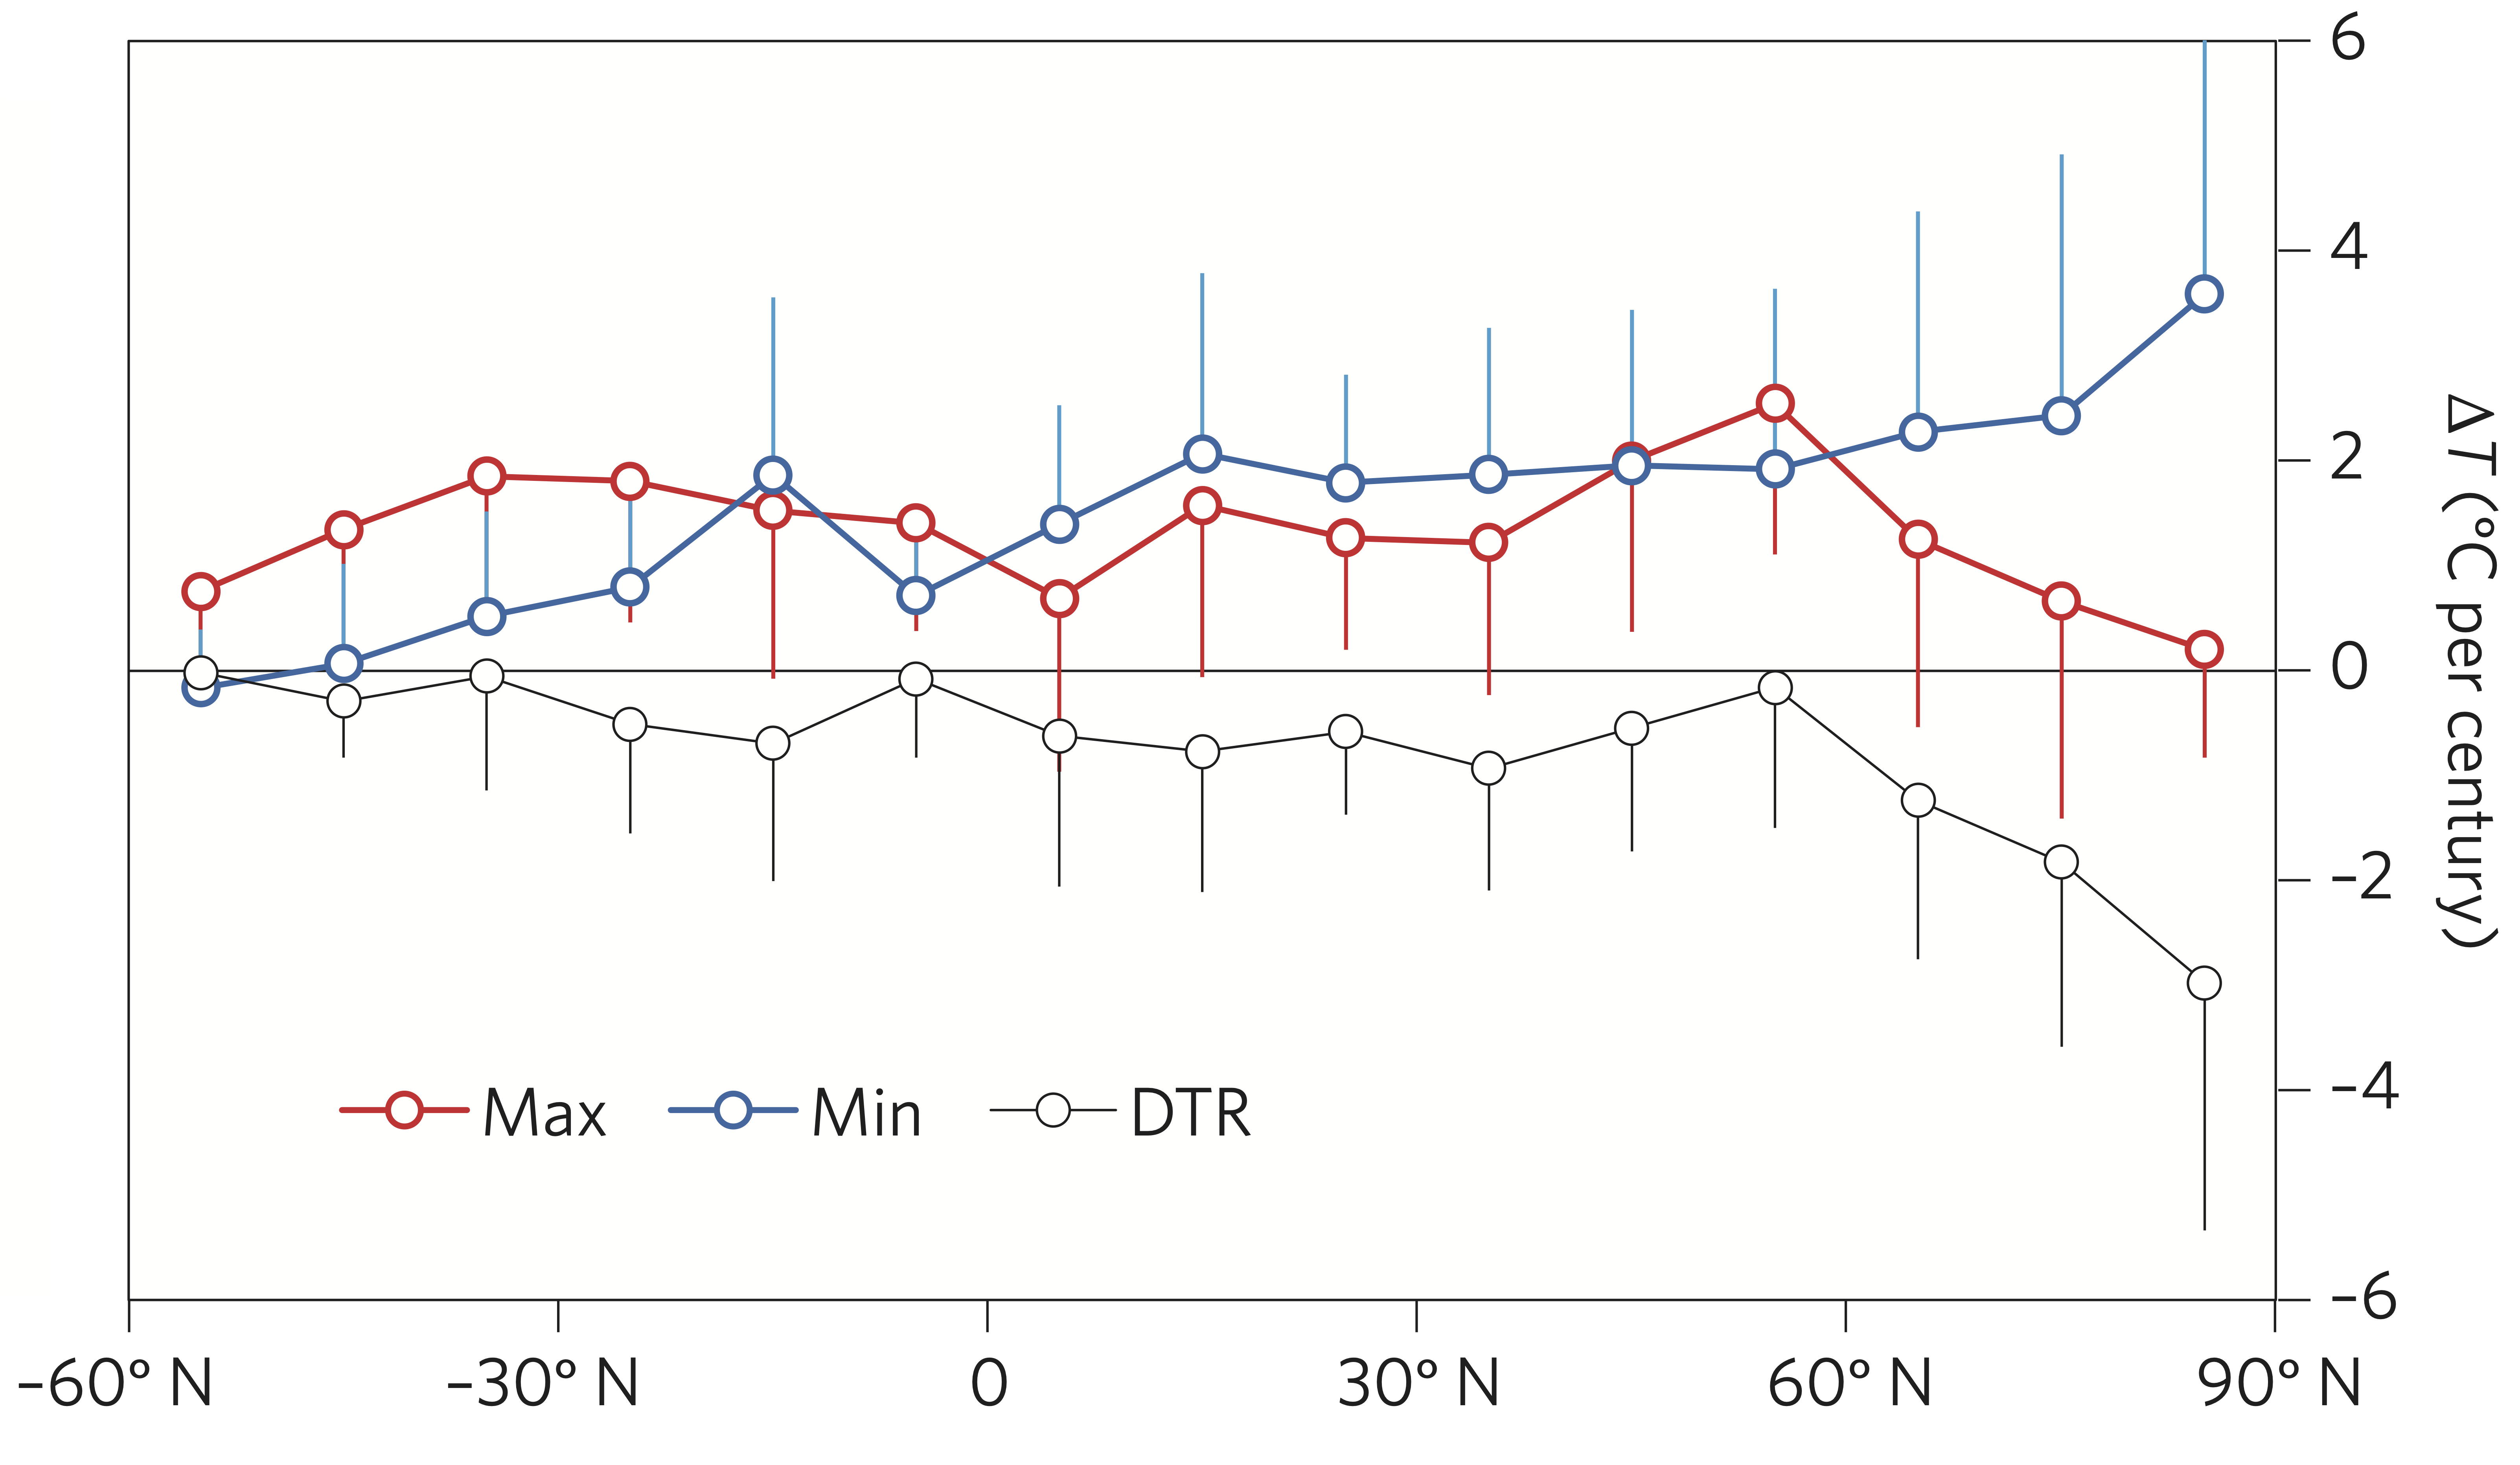
\includegraphics[height=2in]{Figures/xia2014_temp_figure.png}
      \captionof{figure}{The area-weighing rates of temperature change ($\Delta$ T $^{\circ}$C per century) along latitudes with a 10$^{\circ}$ interval (bars represent the standard deviation) over the period 1948 to 2010 (Xia et al., 2014). $\textbf{Max}$- Mean daily maximum temperature, $\textbf{Min}$- Mean daily minimum temperature,  $\textbf{DTR}$- Mean diurnal temperature range.}
      \label{fig:temp_lat}
\end{minipage}
\vspace{0.5em}

\newpage

\subsection{Example 2}
This example has the chapter and figure number in the caption. See the usage of figure width (in LATEX code) to control how the figure is shown.

\begin{minipage}[c]{0.45\textwidth}
    \counterwithin{figure}{section}
    \centering
    \captionsetup{width=.9\linewidth}
    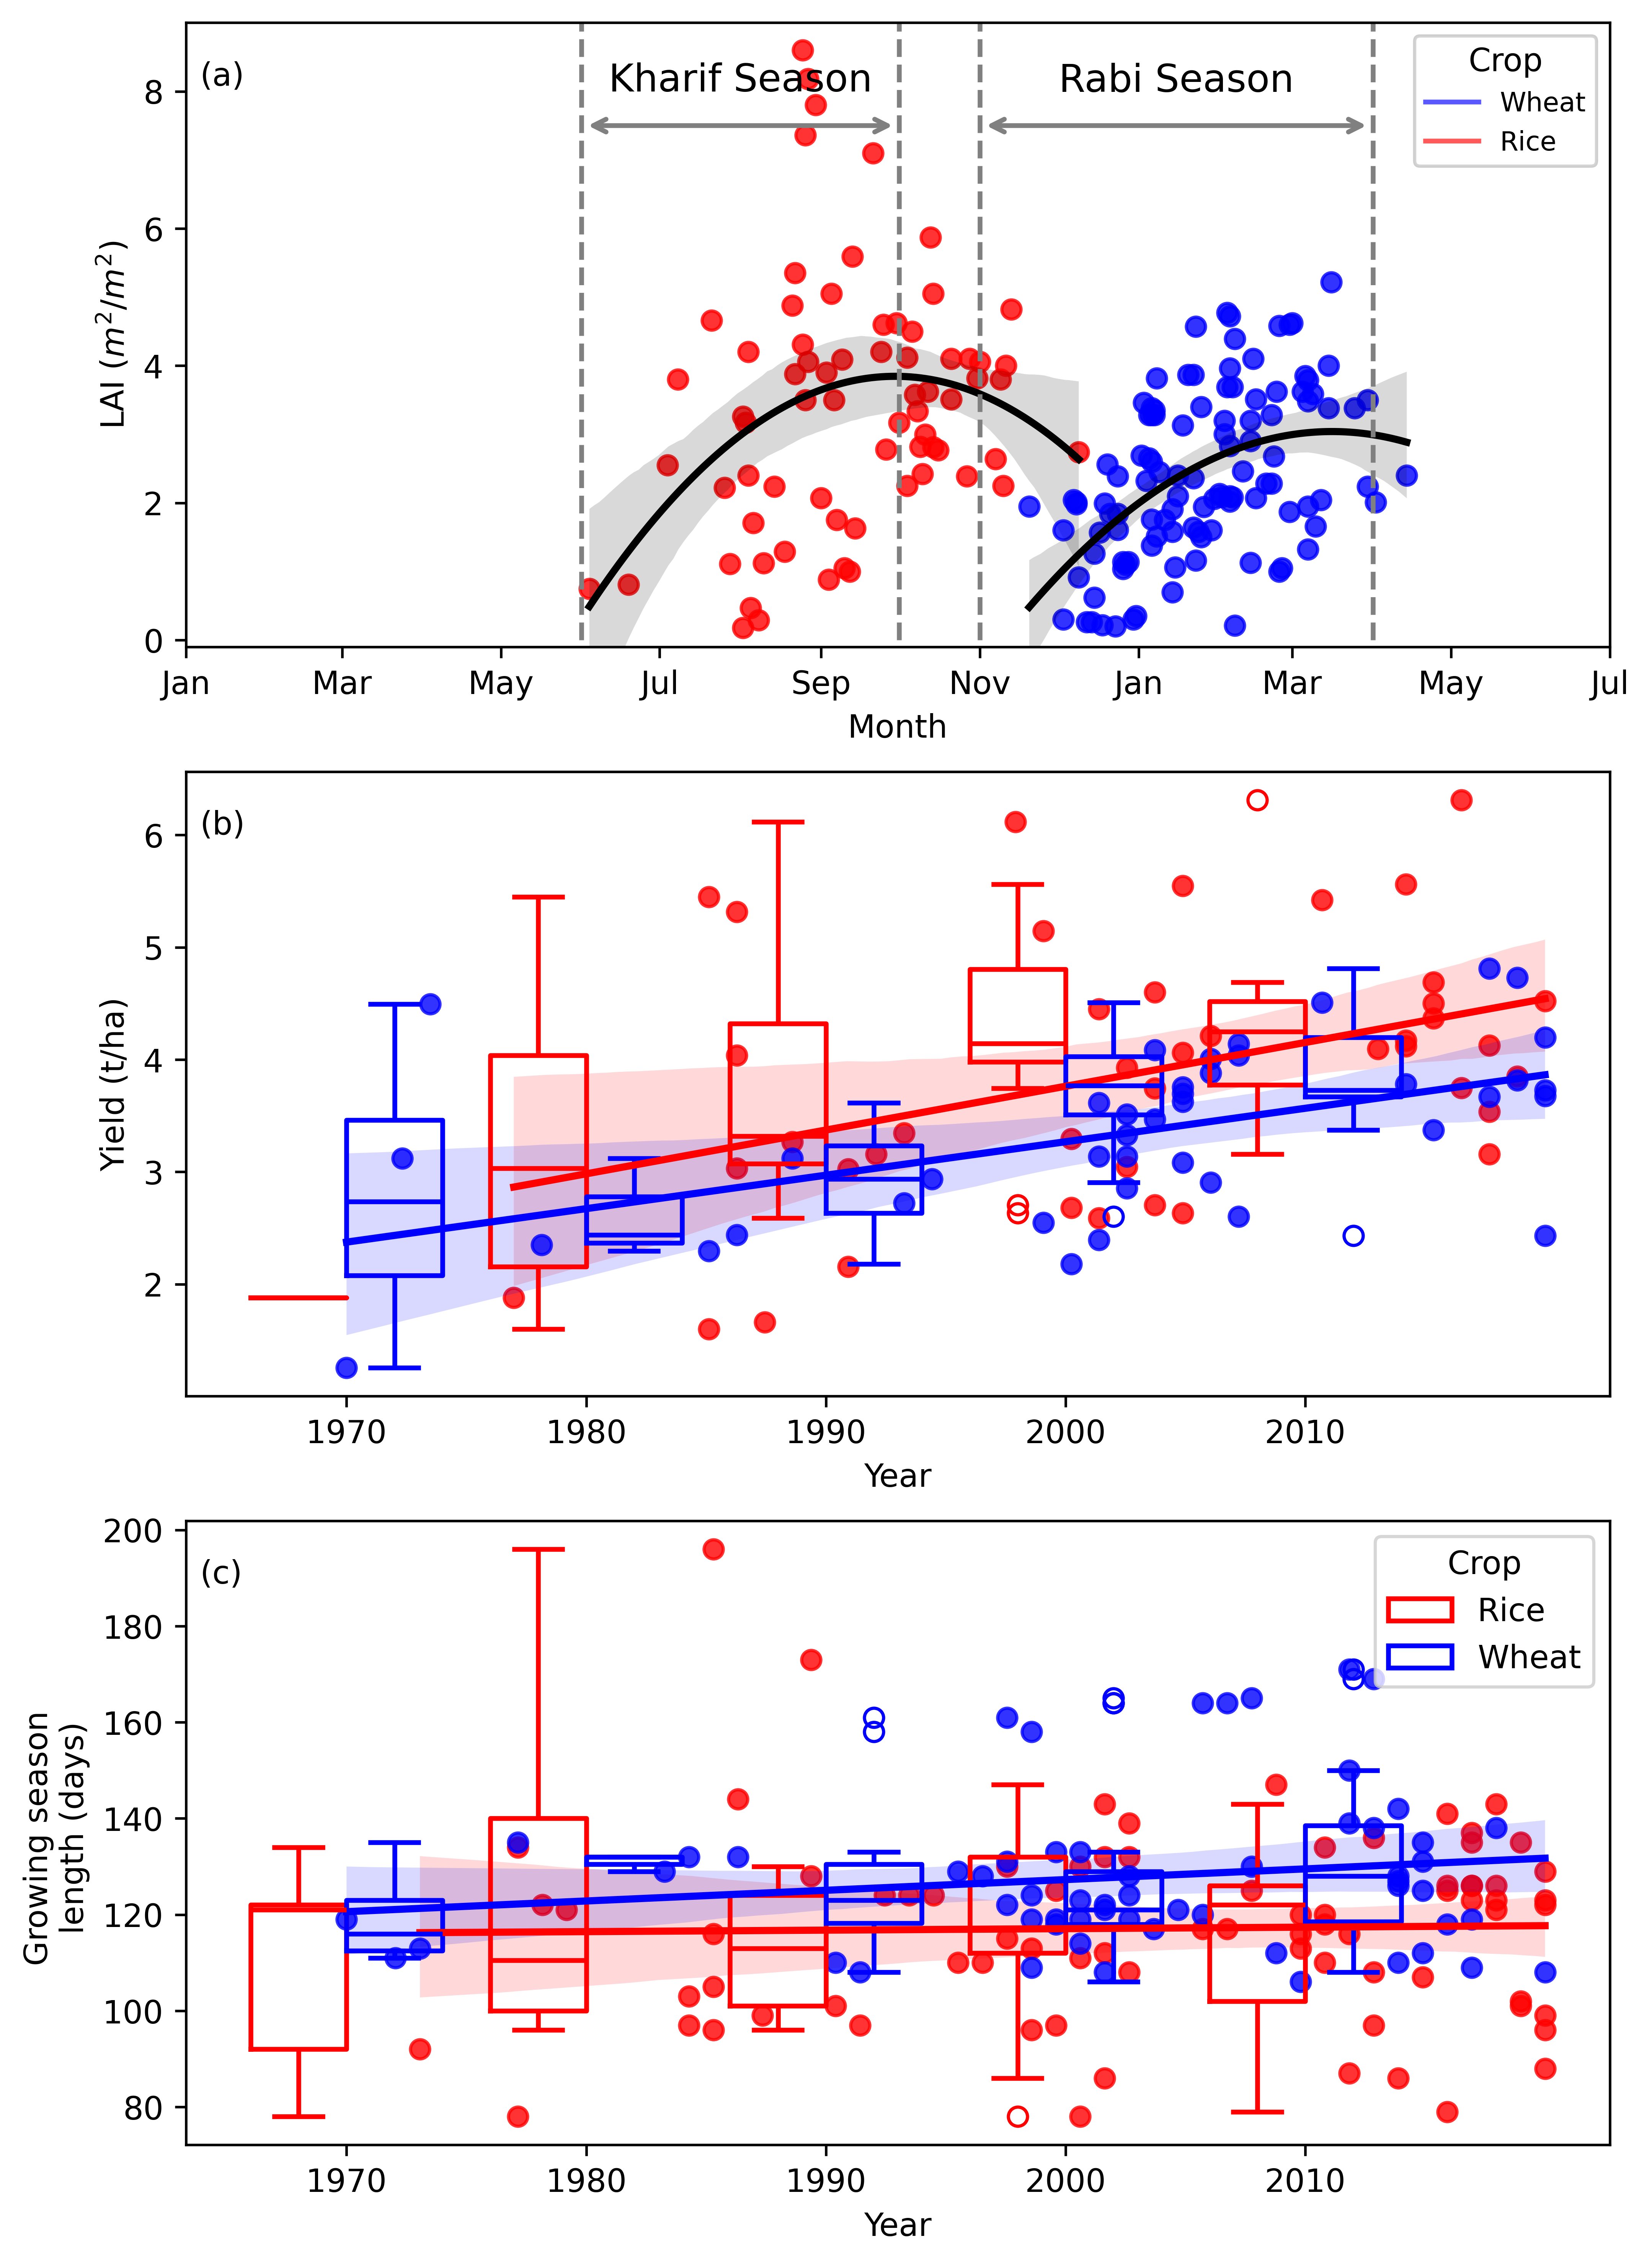
\includegraphics[width=.95\textwidth]{Figures/Analysis_Observation_9Jan.png}
    \captionof{figure}{Analyzing the observational data for (a) LAI, (b) yield, and (c) growing season length in rice and wheat crops.}
    \label{fig:analysis_obs_data}
\end{minipage}
\quad
\begin{minipage}[c]{0.45\textwidth}
    \counterwithin{figure}{section}
    \centering
    \captionsetup{width=.9\linewidth}
    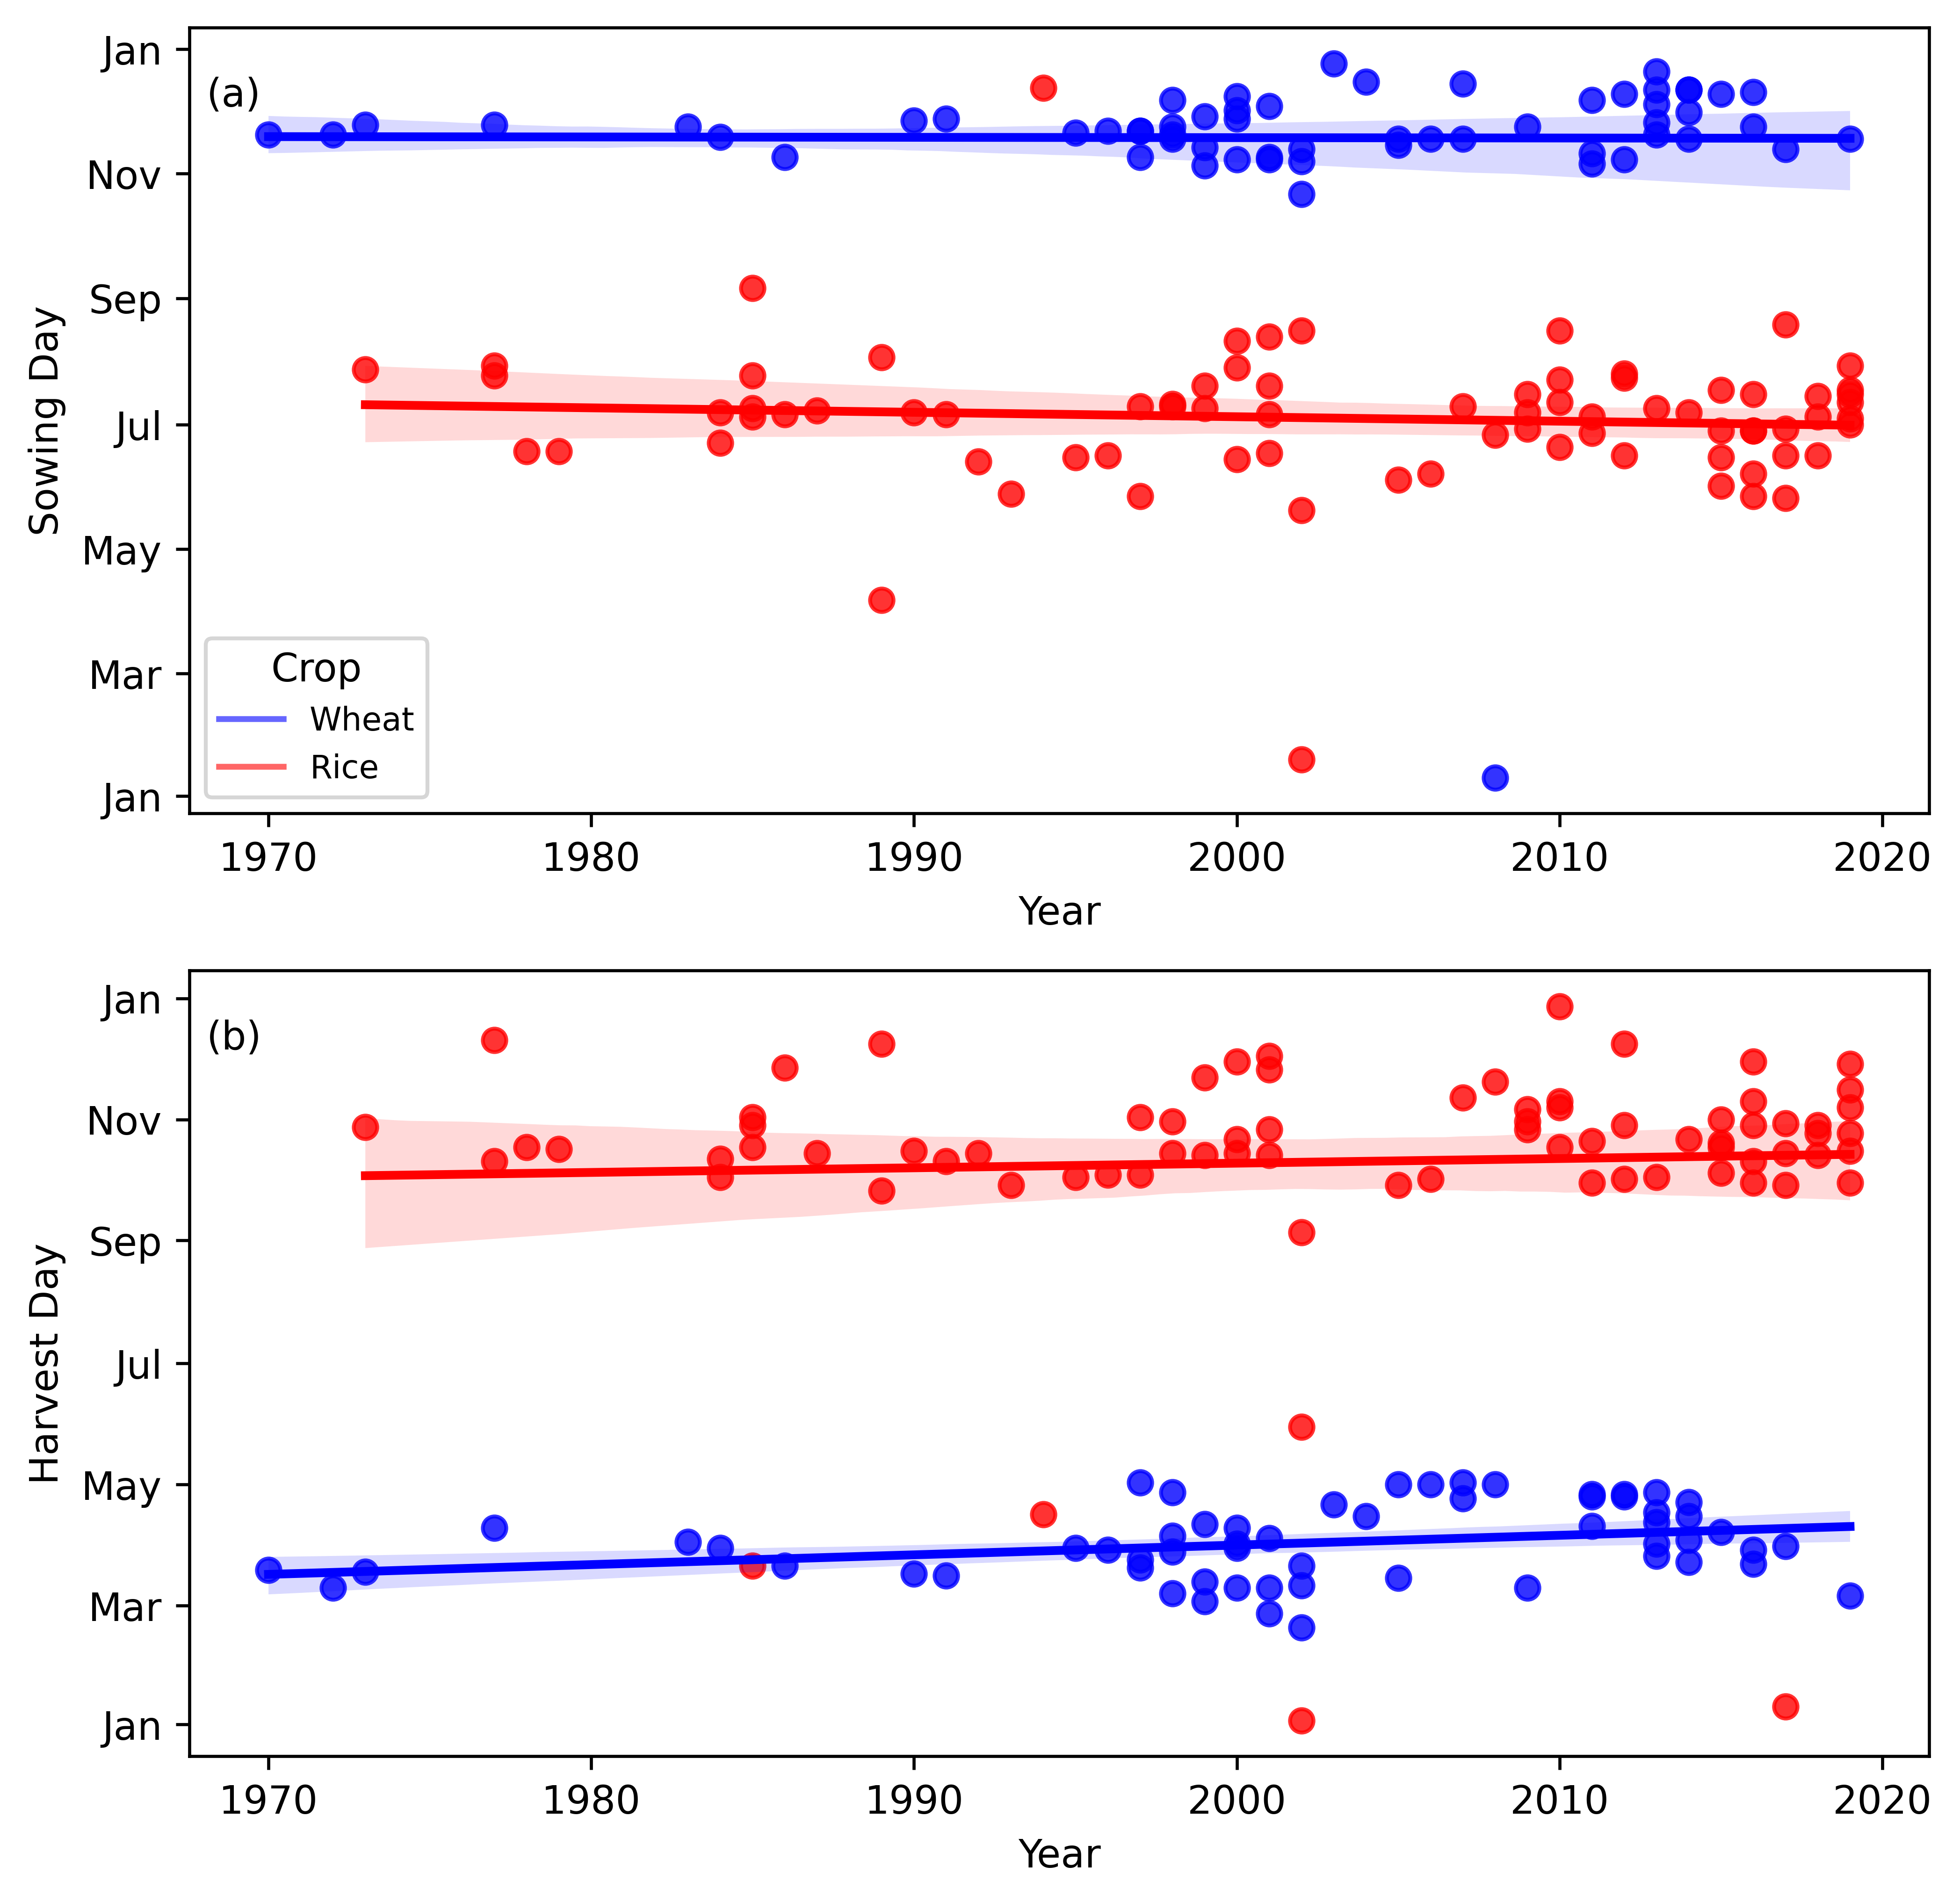
\includegraphics[width=.95\textwidth]{Figures/Analysis_Observation_Sowing_Harvest_Dates_7Jan.png}
    \captionof{figure}{Analyzing the observational data for (a) sowing date  and (b) harvest date in rice and wheat crops.}
    \label{fig:analysis_sow_harv_dates}
\end{minipage}

\section{Complex Tables in LaTeX}

\begin{table}
    \centering
    \counterwithin{table}{section}
    \caption{Table for complex data (multiple rows)}
    \label{tab:Tab21_sitedata_used_for_CLM5}
    \tiny % Reduce font size within the table to prevent overflow
    \begin{tabular}{l l c c c}
        \toprule
        \multicolumn{1}{p{2cm}}{\centering \textbf{Site name}} & \multicolumn{1}{p{3.5cm}}{\centering\textbf{Event ID's in PANGEA repository }} & \multicolumn{1}{p{1.5cm}}{\centering\textbf{Latitude [\textdegree N]}} & \multicolumn{1}{p{1.5cm}}{\centering\textbf{Longitude [\textdegree E]}} & \multicolumn{1}{p{2cm}}{\centering\textbf{Altitude [m] (above sea level)}} \\
        \midrule
        [0.5ex]
        \multirow{\multicolumn{1}{p{2cm}}{{Anantapur}}} & \multicolumn{1}{p{3.5cm}}{{IND\_RI\_RED\_2000}} & \multirow{\multicolumn{1}{p{1.5cm}}{\centering{14.68}}} & \multirow{\multicolumn{1}{p{1.5cm}}{\centering{77.6}}} & \multirow{\multicolumn{1}{p{2cm}}{\centering{350}}} \\ [0.5ex]
         & \multicolumn{1}{p{3.5cm}}{{IND\_RI\_RED\_2001$^*$}} &  &  & \\
         \\
         \multirow{\multicolumn{1}{p{2cm}}{{Cooch Behar}}} & \multicolumn{1}{p{3.5cm}}{{IND\_SW\_COB\_2000}} & \multirow{\multicolumn{1}{p{1.5cm}}{\centering{26.34}}} & \multirow{\multicolumn{1}{p{1.5cm}}{\centering{89.40}}} & \multirow{\multicolumn{1}{p{2cm}}{\centering{43}}} \\ [0.5ex]
         & \multicolumn{1}{p{3.5cm}}{{IND\_SW\_COB\_2001$^*$}} &  &  & \\
         \\
         \multirow{\multicolumn{1}{p{2cm}}{{Faizabad}}} & \multicolumn{1}{p{3.5cm}}{{IND\_SW\_FAZ\_2002}} & \multirow{\multicolumn{1}{p{1.5cm}}{\centering{26.78}}} & \multirow{\multicolumn{1}{p{1.5cm}}{\centering{82.20}}} & \multirow{\multicolumn{1}{p{2cm}}{\centering{113}}} \\ [0.5ex]
         & \multicolumn{1}{p{3.5cm}}{{IND\_SW\_FAZ\_2003}} &  &  & \\ [0.5ex]
         & \multicolumn{1}{p{3.5cm}}{{IND\_SW\_FAZ\_2004$^*$}} &  &  & \\
         \\
         \multirow{\multicolumn{1}{p{2cm}}{{Hyderabad}}} & \multicolumn{1}{p{3.5cm}}{{IND\_RI\_HYD\_2010}} & \multirow{\multicolumn{1}{p{1.5cm}}{\centering{17.19}}} & \multirow{\multicolumn{1}{p{1.5cm}}{\centering{78.23}}} & \multirow{\multicolumn{1}{p{2cm}}{\centering{542}}} \\
         \\
         \multirow{\multicolumn{1}{p{2cm}}{{Jabalpur}}} & \multicolumn{1}{p{3.5cm}}{{IND\_RI\_JAB\_2009}} & \multirow{\multicolumn{1}{p{1.5cm}}{\centering{24.49}}} & \multirow{\multicolumn{1}{p{1.5cm}}{\centering{80.58}}} & \multirow{\multicolumn{1}{p{2cm}}{\centering{412}}} \\ [0.5ex]
         & \multicolumn{1}{p{3.5cm}}{{IND\_RI\_JAB\_2010$^*$}} &  &  & \\ [0.5ex]
         & \multicolumn{1}{p{3.5cm}}{{IND\_RI\_JAB\_2011$^*$}} &  &  & \\
         \\
         \multirow{\multicolumn{1}{p{2cm}}{{Jobner}}} & \multicolumn{1}{p{3.5cm}}{{IND\_SW\_JOB\_2013}} & \multirow{\multicolumn{1}{p{1.5cm}}{\centering{26.08}}} & \multirow{\multicolumn{1}{p{1.5cm}}{\centering{75.34}}} & \multirow{\multicolumn{1}{p{2cm}}{\centering{427}}} \\
         \\
         \multirow{\multicolumn{1}{p{2cm}}{{Kaul}}} & \multicolumn{1}{p{3.5cm}}{{IND\_RI\_KAU\_2008}} & \multirow{\multicolumn{1}{p{1.5cm}}{\centering{29.51}}} & \multirow{\multicolumn{1}{p{1.5cm}}{\centering{76.41}}} & \multirow{\multicolumn{1}{p{2cm}}{\centering{241}}} \\
         \\
         \multirow{\multicolumn{1}{p{2cm}}{{Kuthulia}}} & \multicolumn{1}{p{3.5cm}}{{IND\_RI\_KUT\_2013}} & \multirow{\multicolumn{1}{p{1.5cm}}{\centering{24.30}}} & \multirow{\multicolumn{1}{p{1.5cm}}{\centering{80.15}}} & \multirow{\multicolumn{1}{p{2cm}}{\centering{366}}} \\
         \\
         \multirow{\multicolumn{1}{p{2cm}}{{Ludhiana}}} & \multicolumn{1}{p{3.5cm}}{{IND\_SW\_COB\_2011}} & \multirow{\multicolumn{1}{p{1.5cm}}{\centering{30.93}}} & \multirow{\multicolumn{1}{p{1.5cm}}{\centering{75.87}}} & \multirow{\multicolumn{1}{p{2cm}}{\centering{247}}} \\ [0.5ex]
         & \multicolumn{1}{p{3.5cm}}{{IND\_SW\_LUD\_2012$^*$}} &  &  & \\
         \\
         \multirow{\multicolumn{1}{p{2cm}}{{Meerut}}} & \multicolumn{1}{p{3.5cm}}{{IND\_SW\_MEE\_2011}} & \multirow{\multicolumn{1}{p{1.5cm}}{\centering{29.07}}} & \multirow{\multicolumn{1}{p{1.5cm}}{\centering{77.70}}} & \multirow{\multicolumn{1}{p{2cm}}{\centering{237}}} \\ [0.5ex]
         & \multicolumn{1}{p{3.5cm}}{{IND\_SW\_MEE\_2012}} &  &  & \\ [0.5ex]
         & \multicolumn{1}{p{3.5cm}}{{IND\_SW\_MEE\_2013$^*$}} &  &  & \\
         \\
         \multirow{\multicolumn{1}{p{2cm}}{{Nadia}}} & \multicolumn{1}{p{3.5cm}}{{IND\_SW\_NAD\_2000}} & \multirow{\multicolumn{1}{p{1.5cm}}{\centering{22.88}}} & \multirow{\multicolumn{1}{p{1.5cm}}{\centering{89.00}}} & \multirow{\multicolumn{1}{p{2cm}}{\centering{10}}} \\ [0.5ex]
         & \multicolumn{1}{p{3.5cm}}{{IND\_SW\_NAD\_2000}} &  &  & \\ [0.5ex]
         & \multicolumn{1}{p{3.5cm}}{{IND\_SW\_NAD\_2002}} &  &  & \\ [0.5ex]
         & \multicolumn{1}{p{3.5cm}}{{IND\_SW\_NAD\_2008}} &  &  & \\ [0.5ex]
         & \multicolumn{1}{p{3.5cm}}{{IND\_SW\_NAD\_2009$^*$}} &  &  & \\ [0.5ex]
         & \multicolumn{1}{p{3.5cm}}{{IND\_SW\_NAD\_2013$^*$}} &  &  & \\
         \\
         \multirow{\multicolumn{1}{p{2cm}}{{Pantnagar}}} & \multicolumn{1}{p{3.5cm}}{{IND\_SW\_PAN\_2007}} & \multirow{\multicolumn{1}{p{1.5cm}}{\centering{29.00}}} & \multirow{\multicolumn{1}{p{1.5cm}}{\centering{79.48}}} & \multirow{\multicolumn{1}{p{2cm}}{\centering{244}}} \\ [0.5ex]
         & \multicolumn{1}{p{3.5cm}}{{IND\_SW\_PAN\_2008$^*$}} &  &  & \\ [0.5ex]
         & \multicolumn{1}{p{3.5cm}}{{IND\_RI\_PAN\_2011}} &  &  & \\ [0.5ex]
         & \multicolumn{1}{p{3.5cm}}{{IND\_RI\_PAN\_2012$^*$}} &  &  & \\
         \\
         \multirow{\multicolumn{1}{p{2cm}}{{Parbhani}}} & \multicolumn{1}{p{3.5cm}}{{IND\_SW\_PAR\_2001}} & \multirow{\multicolumn{1}{p{1.5cm}}{\centering{19.27}}} & \multirow{\multicolumn{1}{p{1.5cm}}{\centering{76.78}}} & \multirow{\multicolumn{1}{p{2cm}}{\centering{409}}} \\ [0.5ex]
         & \multicolumn{1}{p{3.5cm}}{{IND\_SW\_PAR\_2005}} &  &  & \\ [0.5ex]
         & \multicolumn{1}{p{3.5cm}}{{IND\_SW\_PAR\_2009$^*$}} &  &  & \\
         \\
         \multirow{\multicolumn{1}{p{2cm}}{{Raipur}}} & \multicolumn{1}{p{3.5cm}}{{IND\_RI\_RAI\_2009}} & \multirow{\multicolumn{1}{p{1.5cm}}{\centering{21.04}}} & \multirow{\multicolumn{1}{p{1.5cm}}{\centering{81.39}}} & \multirow{\multicolumn{1}{p{2cm}}{\centering{293}}} \\
        [0.5ex]
        \bottomrule
    \end{tabular}
    \\ 
    [0.5ex]
    \raggedright\scriptsize{\textit{$^*$Site data used for validation. The remaining data is used for calibration. NOTE: This example shows the usage of multirows where one entry in column 1 has multiple entries in column 2 and others. This is highly useful in reporting data in scientific reports and manuscripts.}}
\end{table}

\begin{sidewaystable}
    \centering
    \counterwithin{table}{section}
    \caption{Table in landscape}
    \label{tab:Tab32_parameter_values_Mod1}
    \footnotesize % Reduce font size within the table to prevent overflow
    \begin{tabular}{l l c c c c}
        \toprule
        \multirow{\multicolumn{1}{p{3.25cm}}{\centering\textbf{Parameter}}} & \multirow{\multicolumn{1}{p{7cm}}{\centering\textbf{Description (units)}}} & \multicolumn{2}{p{6cm}}{\centering\textbf{Wheat}} & \multicolumn{2}{p{6cm}}{\centering\textbf{Rice}} \\
         & & \multicolumn{1}{p{2.5cm}}{\centering\textbf{CLM5\_Def}} & \multicolumn{1}{p{2.5cm}}{\centering\textbf{CLM5\_Mod1}} &  \multicolumn{1}{p{2.5cm}}{\centering\textbf{CLM5\_Def}} & \multicolumn{1}{p{2.5cm}}{\centering\textbf{CLM5\_Mod1}} \\
        \midrule
        [0.5ex]
        \multicolumn{1}{p{3cm}}{\textbf{min\_NH\_planting\_date}} & \multicolumn{1}{p{7cm}}{{Minimum planting date for the northern hemisphere (MMDD)}} & \multicolumn{1}{p{2.5cm}}{\centering 401} & \multicolumn{1}{p{2.5cm}}{\centering 1115 \\ (calibrated in this study)} & \multicolumn{1}{p{2.5cm}}{\centering 101} & \multicolumn{1}{p{2.5cm}}{\centering 701 \\ (calibrated in this study)} \\
        \\
        \multicolumn{1}{p{3cm}}{\textbf{max\_NH\_planting\_date}} & \multicolumn{1}{p{7cm}}{{Maximum planting date for the northern hemisphere (MMDD)}} & \multicolumn{1}{p{2.5cm}}{\centering 615} & \multicolumn{1}{p{2.5cm}}{\centering 1231 \\ (calibrated in this study)} & \multicolumn{1}{p{2.5cm}}{\centering 228} & \multicolumn{1}{p{2.5cm}}{\centering 815 \\ (calibrated in this study)} \\
        \\
        \multicolumn{1}{p{3cm}}{\textbf{min\_planting\_temp}} & \multicolumn{1}{p{7cm}}{{Avergare 5-day daily minimum temperature needed for planting (K)}} & \multicolumn{1}{p{2.5cm}}{\centering 272.15} & \multicolumn{1}{p{2.5cm}}{\centering 283.15 \\ (Rao et al., 2015)} & \multicolumn{1}{p{2.5cm}}{\centering 283.15} & \multicolumn{1}{p{2.5cm}}{\centering 294.15 \\ (Kumar et al., 2023)} \\
        \\
        \multicolumn{1}{p{3cm}}{\textbf{planting\_temp}} & \multicolumn{1}{p{7cm}}{{Avergare 10-day temperature needed for planting (K)}} & \multicolumn{1}{p{2.5cm}}{\centering 280.15} & \multicolumn{1}{p{2.5cm}}{\centering 290.15 \\ (Asseng et al., 2016; Mukherjee et al., 2019)} & \multicolumn{1}{p{2.5cm}}{\centering 294.15} & \multicolumn{1}{p{2.5cm}}{\centering 300.15 \\ (Jat et al., 2019)} \\
        \\
        \multicolumn{1}{p{3cm}}{\textbf{baset}} & \multicolumn{1}{p{7cm}}{{Base Temperature (\textdegree C)}} & \multicolumn{1}{p{2.5cm}}{\centering 0} & \multicolumn{1}{p{2.5cm}}{\centering 5 \\ (Mukherjee et al., 2019; Mehta and Dhaliwal, 2023)} & \multicolumn{1}{p{2.5cm}}{\centering 10} & \multicolumn{1}{p{2.5cm}}{\centering 10 \\ (Thakur et al., 2022)} \\
        \\
        \multicolumn{1}{p{3cm}}{\textbf{grnfill}} & \multicolumn{1}{p{7cm}}{{Grain fill parameter}} & \multicolumn{1}{p{2.5cm}}{\centering 0.6} & \multicolumn{1}{p{2.5cm}}{\centering 0.6 \\ (calibrated in this study)} & \multicolumn{1}{p{2.5cm}}{\centering 0.4} & \multicolumn{1}{p{2.5cm}}{\centering 0.65 \\ (calibrated in this study)} \\
        \\
        \multicolumn{1}{p{3cm}}{\textbf{hydgdd}} & \multicolumn{1}{p{7cm}}{{Growing Degree Days for maturity (\textdegree C-days)}} & \multicolumn{1}{p{2.5cm}}{\centering 1700} & \multicolumn{1}{p{2.5cm}}{\centering 1700 \\ (calibrated in this study)} & \multicolumn{1}{p{2.5cm}}{\centering 2100} & \multicolumn{1}{p{2.5cm}}{\centering 2100 \\ (calibrated in this study)} \\
        \\
        \multicolumn{1}{p{3cm}}{\textbf{baset\_mapping}} & \multicolumn{1}{p{7cm}}{{Parameter to switch on/off latitudinal variation in baset in tropics (available options: \textit{'constant'}; \textit{'varytropicsbylat'})}} & \multicolumn{1}{p{2.5cm}}{\centering 'constant' } & \multicolumn{1}{p{2.5cm}}{\centering 'constant'} & \multicolumn{1}{p{2.5cm}}{\centering 'constant'} & \multicolumn{1}{p{2.5cm}}{\centering 'constant'} \\
        [0.5ex]
        \bottomrule
    \end{tabular}
\end{sidewaystable}

\begin{sidewaystable}
    \counterwithin{table}{section}
    \caption{Creating two tables in a page (in landscape orientation)}
    \label{tab:Tab62_carbonfluxes_comp}
    \footnotesize % Reduce font size within the table to prevent overflow
    \begin{tabularx}{0.95\textwidth}{@{}c l c c c c l@{}}
    %\begin{tabular}{p{1.5cm} p{3cm} p{1.25cm} p{1.25cm} p{1.25cm} p{1.25cm} p{3cm}}
        \toprule
        \textbf{Season} & \textbf{Region/Location} & \textbf{GPP (gC/m$^2$)}& \textbf{TER (gC/m$^2$)} & \textbf{NEP (gC/m$^2$)} & \textbf{TER/GPP} & \textbf{Reference} \\ 
        \midrule
        Mean of (1980-2014) & Indian wheat growing region & 390$\pm$42.5 & 230.03$\pm$26.92 & 160.81$\pm$28.67 & 0.58 &  CLM5\_Rf (This study)\\ [0.5ex]
        Mean of (1980-2014) & Indian wheat growing region & 763$\pm$59.9 & 483.41$\pm$34.26 & 279.6$\pm$36.19 & 0.63 &  CLM5\_Ir (This study)\\ [0.5ex]
        Mean of (1980-2014) & Indian wheat growing region & 335.47$\pm$22.6 & 150.59$\pm$8.02 & 186.66$\pm$17.27 & 0.45 &  ISAM (This study)\\ [0.5ex]
        2009-10 & Meerut, India & $--$ & $--$ & 393.15 & $--$ &  Patel et al. (2011)\\ [0.5ex]
        2007-08 & \multirow{Selhausen, Germany} & 1304$\pm$18 & 676$\pm$29 & 627$\pm$15 & 0.51 & \multirow{Schmidt et al. (2012)}\\ [0.5ex]
        2008-09 & & 1067$\pm$27 & 529$\pm$35 & 537$\pm$12 & 0.49 & \\ [0.5ex]
        2007-08 & \multirow{Shouxian, Huaihe River basin, China} & 1220 & 637 & 583 & 0.52 &  \multirow{Chen et al. (2015)}\\ [0.5ex]
        2008-09 & & 1135 & 623 & 512 & 0.54 &  \\ [0.5ex]
        2009-10 & & 859 & 459 & 451 & 0.53 & \\ [0.5ex]
        2014-15 & Saharanpur, India & 621.47 & 429.17 & 192.30 & 0.69 &  Patel et al. (2021)\\ [0.5ex]
        2013-14 & IARI, New Delhi, India & 888 & 304 & 576 & 0.34 & Kumar et al. (2021)\\ [0.5ex]
        \bottomrule
    \end{tabularx}
    \vspace{1cm}
    \centering
    \counterwithin{table}{section}
    \caption{Second table in a landscape orientation}
    \label{tab:Tab63_carbonfluxes_models}
    \small % Reduce font size within the table to prevent overflow
    \begin{tabularx}{0.485\textwidth}{@{}c c c l@{}}
        \toprule
        \textbf{NPP/GPP} & \textbf{AR/GPP} & \textbf{TER/GPP} & \textbf{References} \\ 
        \midrule
        0.57$\pm$0.045 & 0.43$\pm$0.045 & $-$ & This study (CLM5) \\ [0.5ex]
        0.74$\pm$0.001 & 0.26$\pm$0.001 & 0.5006 & This study (ISAM) \\ [0.5ex]
            &   $\sim$0.3-0.6 &     &   Amthor and Baldocchi (2001) \\ [0.5ex] 
        0.76 & 0.24 & 0.59 & Zhang et al. (2020) \\ [0.5ex]
        0.56 & 0.44 & 0.60 & Aubinet et al. (2009) \\ [0.5ex] 
        0.52 & 0.48 & 0.57 & Aubinet et al. (2009) \\ [0.5ex]
        0.51 & 0.49 & 0.71 & Demyan et al. (2016) \\ [0.5ex]
        0.54 & 0.46 & 0.61 & Moureaux et al. (2008) \\ [0.5ex]
        0.55 & 0.45 & 0.57 & Suleau et al. (2011) \\ [0.5ex]
        0.57 & 0.43 & 0.66 & Wang et al. (2015) \\ [0.5ex]
        \bottomrule
    \end{tabularx}
\end{sidewaystable}

\end{document}
